\documentclass[12pt,a4paper]{article}
\usepackage[paper=a4paper]{geometry}% http://ctan.org/pkg/geometry
\usepackage[english]{babel}
\usepackage[T1]{fontenc}


\usepackage{fancyvrb}
\usepackage{multicol}
\usepackage{lipsum}
\usepackage{setspace}
\usepackage{soul}
\usepackage{fontspec}
\usepackage{background}
\usepackage{xcolor} %for use in color links
\usepackage{colortbl}
\usepackage{caption}
\usepackage{pgfgantt}
\usepackage{graphicx}
\usepackage[yyyymmdd]{datetime}
\usepackage{tikz}
\usetikzlibrary{arrows.meta,shapes,positioning,shadows,trees,calc,tikzmark}
\usepackage{multirow}


\usepackage[edges]{forest}
\usepackage{indentfirst} 
\usepackage{pgfgantt}
\usepackage{rotating}
\usepackage[graphicx]{realboxes}
\usepackage{tocloft}
\usepackage{listings}
\usepackage{csquotes}
\definecolor{mGreen}{rgb}{0,0.6,0}
\definecolor{mGray}{rgb}{0.5,0.5,0.5}
\definecolor{mPurple}{rgb}{0.58,0,0.82}
\definecolor{backgroundColour}{rgb}{0.95,0.95,0.92}



\lstdefinestyle{CStyle}{
    backgroundcolor=\color{backgroundColour},   
    commentstyle=\color{mGreen},
    keywordstyle=\color{magenta},
    numberstyle=\tiny\color{mGray},
    stringstyle=\color{mPurple},
    basicstyle=\footnotesize,
    breakatwhitespace=false,         
    breaklines=true,                 
    captionpos=b,                    
    keepspaces=true,                 
    numbers=none,                    
    numbersep=5pt,                  
    showspaces=false,                
    showstringspaces=false,
    showtabs=false,                  
    tabsize=2,
    language=C
}



\newcommand{\listappendicesname}{Appendices}
\newlistof{appendices}{apc}{\listappendicesname}
\newcommand{\appendices}[1]{\addcontentsline{apc}{appendices}{#1}}

\newcommand{\newappendix}[1]{\section*{#1}\appendices{#1}}


\usepackage{sectsty}
\usepackage{float}

\sectionfont{\fontsize{24pt}{36}\selectfont}
\usepackage{tocloft}
\renewcommand{\cftsecleader}{\cftdotfill{\cftdotsep}}
\usepackage{afterpage}

\usepackage{listings}
\usepackage{color}
 
\definecolor{codegreen}{rgb}{0,0.6,0}
\definecolor{codegray}{rgb}{0.5,0.5,0.5}
\definecolor{codepurple}{rgb}{0.58,0,0.82}
\definecolor{backcolour}{rgb}{0.95,0.95,0.92}
 
\lstdefinestyle{mystyle}{
    backgroundcolor=\color{backcolour},   
    commentstyle=\color{codegreen},
    keywordstyle=\color{magenta},
    numberstyle=\tiny\color{codegray},
    stringstyle=\color{codepurple},
    basicstyle=\footnotesize,
    breakatwhitespace=false,         
    breaklines=true,                 
    captionpos=b,                    
    keepspaces=true,                 
    numbers=left,                    
    numbersep=5pt,                  
    showspaces=false,                
    showstringspaces=false,
    showtabs=false,                  
    tabsize=2
}
 
\lstset{style=mystyle}
\captionsetup{justification=raggedright,singlelinecheck=false}

\newcommand\blankpage{%
    \null
    \thispagestyle{empty}%
    \addtocounter{page}{-1}%
    \newpage}
\renewcommand{\baselinestretch}{1.5} 

\usetikzlibrary{calc}
\newcommand\HRule{\rule{\textwidth}{1pt}}

\setmainfont[Ligatures=TeX]{Times New Roman}
\newgeometry{top=25mm,bottom=40mm,left=40mm,right=25mm}
\usepackage[nottoc,numbib]{tocbibind}

\backgroundsetup{
color=black,
scale=1,
opacity=1,
angle=0,
contents={
\begin{tikzpicture}
\draw [line width=0.75pt] ($ (current page.north west) + (2.5cm,-1cm) $) rectangle ($ (current page.south east) + (-1cm,1cm) $);
\draw [line width=0.01pt] ($ (current page.north west) + (0cm,0cm) $) rectangle    ($ (current page.south east) + (0cm,0cm) $); 
\end{tikzpicture}
}
}

\setlength{\footskip}{20pt}


\begin{document}

\begin{titlepage}
\begin{tikzpicture}[remember picture, overlay]
\draw [line width=0.75pt] ($ (current page.north west) + (2.5cm,-1cm) $) rectangle ($ (current page.south east) + (-1cm,1cm) $);
\draw [line width=0.01pt] ($ (current page.north west) + (0cm,0cm) $) rectangle    ($ (current page.south east) + (0cm,0cm) $); 
\end{tikzpicture}

\begin{flushright}
\textbf{\uppercase{\fontsize{12}{18} \selectfont {Group No: 1}}}
\end{flushright}


\center % Center everything on the page
{\setstretch{1.2}
\includegraphics[width=1.8in,height=1.8in,keepaspectratio]{logo.png}\\[0.5cm]
\fontsize{16pt}{24}\selectfont \textbf{Project Report}\\[0.5cm]
% \fontsize{16pt}{24}\selectfont \textbf{ETE 2112}\\[0.75cm]
\fontsize{24pt}{30}\selectfont \textbf{\uppercase{Vertical Axis Wind Turbines}}\\[0.5cm]
\fontsize{16pt}{24}\selectfont \textbf{By}\\[0.5cm]


\vspace*{\fill}
\fontsize{12pt}{12}\selectfont {
\bgroup
\def\arraystretch{1.4}% 
\begin{tabular}{|c|l|c|}
        \hline
        \textbf{Index No} &        \textbf{Name} \\ 	\hline 
        EGT/16/403 & Alagiyawanna A.M.A.K.M. \\ 					\hline
        EGT/16/409 & Balasuriya B.M.C.M. \\ 					\hline
        EGT/16/418 & Chathumini K.K.G.L. \\ 					\hline
        EGT/16/419 & Dassanayake N.P. \\ 					\hline
        EGT/16/421 & Dewasurendra J.W \\ 					\hline
        EGT/16/425 & Dissanayake H.D.S.C.  \\			\hline
        EGT/16/437 & Gnanakeethan B.  \\				\hline
        EGT/16/442 & Hansa R.Y.D. \\ 					\hline
        EGT/16/451 & Imtiyaz F.A.  \\        			\hline
        EGT/16/461 & Kamalka H.A.B.  \\         		\hline

\end{tabular}
\egroup
}\\[0.5cm]

\vspace*{\fill}

\fontsize{12pt}{12}\selectfont \textbf {Department of Engineering Technology \\ Faculty of Technology\\University of Sri Jayewardenepura\\ Sri Lanka}\\[0.5cm]
}

\vspace*{\fill}

\end{titlepage}


\newpage 
\pagenumbering{roman}
\renewcommand{\baselinestretch}{1}\normalsize
\tableofcontents

% \cleardoublepage
% \phantomsection
% \addcontentsline{toc}{chapter}{\listfigurename}

\newpage

\pagenumbering{arabic}
%\pagenumbering{gobble}
\setcounter{page}{1}
%\addcontentsline{toc}{section}{Unnumbered Section}

\setcounter{secnumdepth}{3}
\renewcommand{\baselinestretch}{1.5}\normalsize


\section{Introduction}
Most wind turbines fall into one of two general categories: horizontal axis and vertical axis. Each can be further divided into small and large wind turbines.

\newpage

\section{Vertical axis wind turbines}
Vertical axis wind turbines (or VAWTs) have the main rotor shaft arranged vertically. Key advantages of this arrangement are that the turbine does not need to be pointed into the wind to be effective. This is an advantage on sites where the wind direction is highly variable. VAWTs can utilize winds from varying directions. With a vertical axis, the generator and gearbox can be placed near the ground, so the tower doesn’t need to support it, and it is more accessible for maintenance. Drawbacks are that some designs produce pulsating torque. Drag may be created when the blade rotates into the wind.
It is difficult to mount vertical-axis turbines on towers, meaning they are often installed nearer to the base on which they rest, such as the ground or a building rooftop. The wind speed is slower at a lower altitude, so less wind energy is available for a given size turbine. Air flow near the ground and other objects can create turbulent flow, which can introduce issues of vibration, including noise and bearing wear which may increase the maintenance or shorten the service life.
However, when the turbine is mounted on a rooftop, the building generally redirects wind over the roof and this can double the wind speed at the turbine. If the height of the rooftop mounted turbine tower is approximately 50 percent of the building height, this is near the optimum for maximum wind energy and minimum wind turbulence

\newpage 
\section{Working mechanism}
The rotational movement of the blade generates a head wind that combines with the actual wind to form the apparent wind. If the angle of this apparent wind on the blade is larger than zero, the lift force has a forward component that propels the turbine. 
The angle of attack which varies in a revolution between -20 to +20 should not exceed 20 degrees since at higher angles the flow along the blade is no longer laminar, which is a condition required for the generation of a lift force, but becomes turbulent causing stall. 
The original designs suffered from some negative features such as violent vibrations leading to eventual fatigue blade failure, a high noise level and a relatively low efficiency, which severely limited the success of the vertical wind turbines. 

\newpage
\section{Types of vertical wind turbines}
\subsection{Classified on size}
\subsubsection{Small vertical axis wind turbines}
Small vertical axis wind turbines differ greatly from middle to large vertical axis wind turbines because a blade’s driving force and direction are different when a blade rotates. At some position, the blade force is big and the direction are positive. At some positions, the driving force will be smaller and also positive. But at other positions, the driving force and direction are negative, and big and small. Also, as the rotor diameter is made bigger, the negative forces become larger. So if the diameter of the rotor is made larger, the blade’s angle (pitch) has to be adjustable in real time. This is called “real time attack angle control regulation” technology.
\subsubsection{Medium \& large VAWT technologies}
Though many other turbine manufacturers are developing medium and large VAWT, they have adopted the design approach from small VAWTs by simply proportionally enlarging a small turbine to become a “medium or large VAWT”. They do not truly understand the characteristics of a VAWT.
It is well known that a VAWT is quiet, safe, and does not need a tall tower. However, hardly any commercialized large VAWT have been launched despite the efforts of countless engineers. The reasons are obvious: the problems of aerodynamic efficiency, self-starting, structural stability, and safe braking remain unsolved. The problems have to be solved for any type of wind turbine.

\subsection{Classified based on blade shape}
\subsubsection{Darrieus}
Georges Darrieus was the French inventor of the Darrieus vertical-axis wind turbine or 'eggbeater windmill' in 1931 – manufactured by FloWind (no longer trading) for North American customers. A Darrieus is a high speed, low torque machine suitable for generating alternating current (AC)electricity. The device develops lift from 2 or 3 'C' shaped blades. A Darrieus is unable to self-starter, which necessitates either a manual push or a more elaborate starter mechanism.
 
 
 
 
\subsubsection{Giromill}
A Giromill (also known as an 'eggbeater windmill') uses the same principal as a Darrieus to capture wind energy, but uses 2 or 3 straight blades individually attached to a vertical axis.
 
 
\subsubsection{Helical Blades}
By replacing the blades of a Giromill with helical blades wrapped around a vertical axis (in a DNA-like structure), it is possible to minimize the pulsating torque that can cause the main bearings to fail on Darrieus-derived designs.
The original idea for this wind turbine was inspired by the Gorlov Helical Water Turbine, which in turn was originally inspired by the Darrieus wind turbine design.
 
 
\subsubsection{Cycloturbine}
Yet another variation of the Darrieus is the Cycloturbine, which is essentially a Giromill with variable angle-of-attack blades. By varying the blade angle as it rotates against the wind, the blade drag is minimized. This modification improves the overall efficiency of the device, but also increases its complexity. Also varying the blade angle during startup reduces the startup torque required and avoids the need for a starter.
\subsubsection{Savonius}
A Savonius vertical-axis wind turbine is a slow rotating, high torque machine that is ideal for driving pumps. Whereas most wind turbines use lift generated by airfoil-shaped blades to drive a rotor, the Savonius uses drag and therefore cannot rotate faster than the approaching wind speed.
 
To feed the electricity grid, the relatively slow speed of a Savonius needs to be geared up to produce AC frequencies – increasing cost and reducing overall efficiency.

\newpage
\section{Advantages of Vertical Axis Wind Turbines}
\begin{itemize}
\item They can produce electricity in any wind direction.
\item Strong supporting tower is not needed because generator, gearbox and other components are placed on the ground.
\item Low production cost as compared to horizontal axis wind turbines.
\item As there is no need of pointing turbine in wind direction to be efficient so yaw drive and pitch mechanism is not needed.
\item Easy installation as compared to other wind turbine.
\item Easy to transport from one place to another.
\item Low maintenance costs.
\item They can be installed in urban areas.
\item Low risk for humans and birds because blades moves at relatively low speeds.
\item They are particularly suitable for areas with extreme weather conditions, like in the mountains where they can supply electricity to mountain huts.
\item Lower wind power is needed to generate electricity
\end{itemize}


\newpage
\section{Disadvantages of Vertical Axis Wind Turbines}
\begin{itemize}
\item As only one blade of a wind turbine works at a time, efficiency is very low compared to HAWTS.
\item They need an initial push to start; this initial push that to make the blades start spinning on their own must be started by a small motor.
\item When compared to horizontal axis wind turbines they are very less efficient because of the additional drag created when their blades rotate.
\item They have relative high vibration because the air flow near the ground creates turbulent flow.
\item Because of vibration, bearing wear increases which results in the increase of maintenance costs.
\item They can create noise pollution.
\item VAWTs may need guy wires to hold it up (guy wires are impractical and heavy in farm areas)
\item Complicated structure
\item Stress on blades due to centrifugal force
\item Fatigues on blades
\item Very low starting torques
\item Problems in dynamic stability
\end{itemize}




% 
\end{document}
